% TODO:
% - Listing verbessern (Größe, evtl. Hintergrundfarbe)
% - Listings besser anordnen



% \lstinputlisting[frame=single, float, caption={CAPTION ???}, label={lst:preproc}, firstline=25, lastline=30]{../../../Programming/miscStuff/coin_count/coin.m}

\documentclass[a4paper,DIV=calc,ngerman]{scrartcl}

\usepackage[utf8]{inputenc}
\usepackage[T1]{fontenc}
\usepackage[ngerman]{babel}
\usepackage{setspace}
\usepackage{microtype}
\usepackage{lmodern}
\usepackage{listings}					% Code-Abschnitt mit Syntax-Highlighting
\lstset{
language=matlab,
%breaklines=true,
%breakatwhitespace=true
basicstyle=\footnotesize,
numbers=left,
numberstyle=\footnotesize,
stepnumber=2,
numbersep=5pt,
extendedchars=true,					% Macht das überhaupt was???
inputencoding=utf8,
breakindent=30pt,
escapeinside={\%(}{\%)},
captionpos=b
%xleftmargin=20pt					% Einrückung der listings
}
\usepackage[pdftex]{graphicx}
\graphicspath{{images/}}
\usepackage{wrapfig}
\usepackage[
  pdftex,
  bookmarks, bookmarksopen, bookmarksopenlevel=1, bookmarksnumbered=true,
  pdfpagemode={UseNone},
  pdfpagelayout={SinglePage},
  plainpages=false,
  pdfkeywords={Bildverarbeitung},
  pdfsubject={Bildverarbeitung},
  pdftitle={Bildverarbeitung},
  pdfauthor={Martin Wichmann}
]{hyperref}
\usepackage{booktabs}


\hyphenation{}

\begin{document}

\titlehead{\center{\large \textsc{Ostfalia Hochschule für angewandte Wissenschaften}}}
\title{Bildverarbeitung}
\author{Martin Wichmann\\701\,277\,37}
\date{\today}

\maketitle
\tableofcontents

% TODO: schauen ob text auch auf erste sein soll?!
\thispagestyle{empty}

\newpage
\setcounter{page}{1}

%%%%%%%%%%%%%%%%%%%%%%%%%%%%%%%%%%%%%%%%%%%%%%%%%%%%%%%%%%%
% Worum gehts eigentlich...
\section{Einleitung}
\label{sec:Einleitung}
Diese Ausarbeitung dokumentiert zwei Aufgaben aus dem Bereich der Bildverarbeitung. Neben den ausgearbeiteten Lösungsansätzen werden mögliche Erweiterungen und Verbesserungen betrachtet. Dabei werden die theoretischen Grundlagen der Bildverarbeitung vorausgesetzt und nicht näher erläutert.

Bei der ersten Aufgabe handelt es sich um einen Münzenzähler. Hierbei soll ein Bild ausgewertet werden und untersucht werden welche und wie viele Münzen zu sehen sind. Die Lösung hierzu wurde in Matlab\footnote{Matlab Version 2011b inklusive Image Processing Toolbox} erstellt.

Aufgabe 2 betrachtet ein Video einer, auf einem Modellauto plazierten, Web-Cam. Die Auswertung der Bilder soll hier die Seitenlinien und Stopplinien erkennen und somit Kurven und Kreuzungen erkennen. Diese Aufgabe wurde mithilfe von OpenCV bearbeitet. Dabei wurde Python als Programmiersprache gewählt.

Dieses Dokument enthält lediglich relevante Code-Abschnitte. Der gesamte Quellcode wurde auf GitHub\footnote{Münzenzähler: \url{https://github.com/erebos42/miscStuff/tree/master/coin_count} und Farhbahnerkennung: \url{https://github.com/erebos42/miscStuff/tree/master/BV_1}} hoch geladen und ist frei verfügbar.




%%%%%%%%%%%%%%%%%%%%%%%%%%%%%%%%%%%%%%%%%%%%%%%%%%%%%%%%%%%
% Aufgabe 1 - Münzenzähler
\section{Aufgabe 1 - Münzenzähler}
\label{sec:aufgabe1}
In dieser Aufgabe wird mittels Matlab ein Bild ausgewertet und die Anzahl und Zusammenstellung der Münzen ausgegeben. Da im Originalbild zwei Münzen zu nah beieinander lagen um gut erkannt werden zu können, wurde dieses Bild mittels Gimp von Hand verändert.


\subsection{Allgemeine Idee}
\label{sec:a1idee}
Die grundsätzliche Vorgehensweise bei dieser Aufgabe kann auf folgende Punkte aufgeteilt werden:

\begin{enumerate}
    \item Bild laden
    \item Bild aufbereiten
    \item Objekte erkennen
    \item Münzen erkennen
\end{enumerate}

Im ersten Punkt wird das Bild in Matlab geladen. Hierdurch kann weiter mit dem Bild gearbeitet werden. Im nächsten Schritt wird das Bild aufbereitet. Dies ist nötig da ansonsten Bild-Rauschen und -Fehler die Objekterkennung erschweren würden. In diesem Zusammenhang wird vor allem auf Erosion und Dilatation zurückgegriffen. Außerdem wird ein Kantendetektions-Filter angewendet.

Nachdem das Bild nun vorbereitet wurde werden alle Objekte im Bild erkannt. Dabei wird auf eine Matlab-Funktionen zurückgegriffen. Zu guter Letzt werden die Münzen anhand ihrer Eigenschaften unterschieden.

Zwischen allen relevanten Schritten wird das aktuelle Bild ausgegeben um den Ablauf nachvollziehen zu können. Das fertige Ergebnis ist in Abbildung \ref{fig:coincountresult} zu sehen.


\begin{figure}
\centering
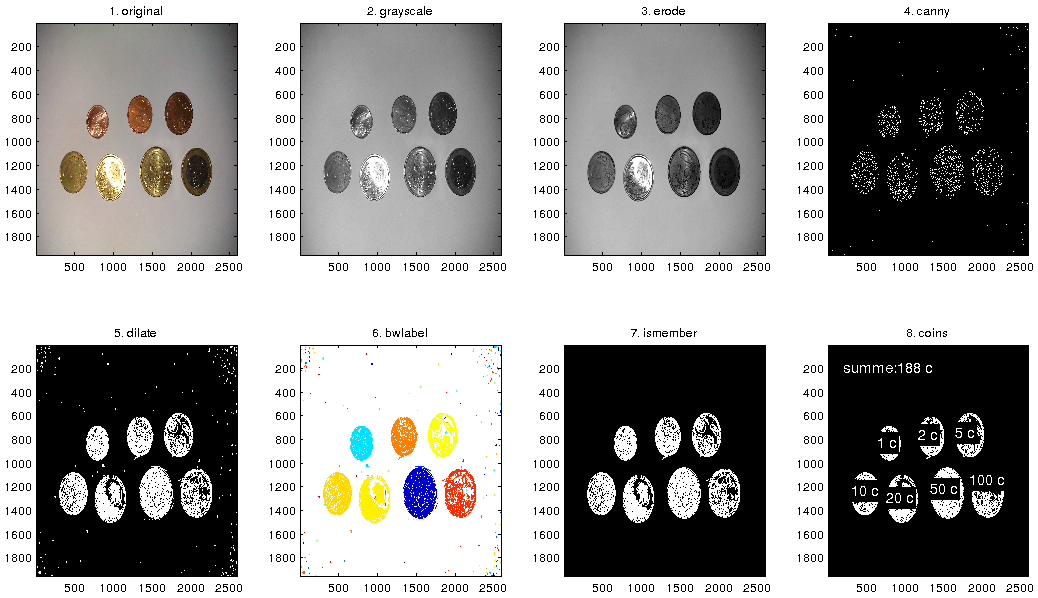
\includegraphics[width=13cm]{coin_count_result2}
\caption{Münzenzähler Ergebnis}
\label{fig:coincountresult}
\end{figure}



\subsection{Umsetzung}
\label{sec:a1umsetzung}
Im folgenden werden relevante Ausschnitte aus dem Quellcode erläutert.

\begin{lstlisting}[frame=single, float, caption={Bild einlesen}, label={lst:bildeinlesen}]
colormap('Gray');
Irgb=imread('IMAG0092_improved.jpg');
Ibw=rgb2gray(Irgb);
\end{lstlisting}

In Listing \ref{lst:bildeinlesen} wird das Bild eingelesen und in einer Variable gespeichert. Dabei wird in der letzten Zeile das Bild in ein Grauton-Bild gewandelt. Dies ist hilfreich, da im weiteren die Farbwerte keine Rolle spielen und außerdem die Operationen einfacher durchzuführen sind.

\begin{lstlisting}[frame=single, float, caption={Bild-Aufbereitung}, label={lst:bildaufbereitung}]
SE=ones(3,3);

Itemp=imerode(Ibw,SE);
Itemp=imerode(Itemp,SE);

Itemp=edge(Itemp,'canny',0.03);

Itemp=imdilate(Itemp,SE);
Itemp=imdilate(Itemp,SE);
\end{lstlisting}

Listing \ref{lst:bildaufbereitung} befasst sich mit dem Aufbereiten des Bilds. Dabei wird auf die Erosion und Dilatation zurückgegriffen. Außerdem wird in Zeile 6 ein Canny-Kantenfilter eingesetzt. Dieser komplette Abschnitt wurde mittels "`trial and error"' entworfen, da es viele Wege gibt um das Bild zu optimieren. Weitere Möglichkeiten der Verbesserung wären zum Beispiel das Einsetzen von Opening und Closing oder der Einsatz von anderen Kanten-Filtern. Es wäre auch möglich das Bild mittels einer einfachen Schwelle in ein Zweipegel-Bild umzuwandeln oder andere Filter einzusetzen. Die Bild-Qualität ist jedoch bei komplexeren Filtern nicht unbedingt besser, und so bietet es sich an eine möglichst einfache Variante zu verwenden. Wie sich in den nächsten Schritten herausstellte, war die Bild-Qualität nach der angewendeten Aufbereitung ausreichend.


\begin{lstlisting}[frame=single, float, caption={Objekt-Segmentierung}, label={lst:segmentierung}]
L=bwlabel(Itemp);
col=label2rgb(L,'jet','w','shuffle');
\end{lstlisting}

Nachdem Bild-Rauschen und andere Fehlern minimiert wurden, können nun die Objekte segmentiert werden. Der zugehörige Quellcode ist in Listing \ref{lst:segmentierung} zu sehen. Hierfür wird in Zeile eins eine einzige Matlab-Funtion eingesetzt. Diese implementiert eine abgewandelte Form eines Floodfill-Algorithmus. Bei dieser Variante wird das Bild Lauflängen-Codiert.\cite{1} Anschließend werden den Läufen vorläufige Labels zugeordnet und im nächsten Schritt zu den endgültigen Labels gewandelt. Zeile zwei des Listings färbt die segmentierten Objekte zufällig ein.


\begin{lstlisting}[frame=single, float, caption={Objekt-Klassifizierung}, label={lst:klassifizierung}]
props=regionprops(L,'Area');

area=[props.Area];
ObjArea=find(area > 10000);

mask=ismember(L, ObjArea);
\end{lstlisting}
Die Objekt-Klassifizierung findet in Listing \ref{lst:klassifizierung} statt. Hier werden in Zeile eins die Eigenschaften, hier nur die Fläche, der vorher erkannten Objekte bestimmt. Diese Flächen werden in Zeile drei in einen Vektor geschrieben und in Zeile vier anhand eines Schwellwerts gefiltert. Die letzte Zeile in diesem Listing wählt nur die Objekte (Pixel) aus, die auch den gewählten Eigenschaften entsprechen. 

\begin{lstlisting}[frame=single, float, caption={Münzen-Erkennung}, label={lst:detectcoins}]
for i = ObjArea
    [r, c] = find(L==i);
    
    if ((area(i) >= 55000) && (area(i) <= 65000))
        z = 1;
    elseif ((area(i) >= 65001) && (area(i) <= 70000))
        z = 5;
    ...
    else
        z = 0;
    end

    cointext = strcat(num2str(z), ' c');
    text(c(1),r(1),cointext);
end
\end{lstlisting}

Die abschließende Münzen-Erkennung ist in Listing \ref{lst:detectcoins} zu finden. Die for-Schleife wird dabei genutzt um über alle erkannten Objekte zu iterieren. Anschließend werden in Zeile zwei alle Pixel ermittelt, die zu diesem Objekt gehören. Das darauf folgende if-Konstrukt wird verwendet um anhand der Fläche die Münzen zu unterscheiden. Die dabei angegebenen Grenzwerte wurden von Hand für dieses Bild ermittelt und müssten für andere Bilder angepasst werden. In den Zeilen 13 und 14 werden nun ein Textfeld ins Bild gesetzt das angibt welchen Wert die Münze hat.

Vor allem in diesem Schritt ist es möglich umfangreiche Verbesserungen einzubauen. So könnte zusätzlich ein Referenz-Objekt mit aufgenommen werden, um so die Schwellwerte für die Münzen automatisch ermitteln zu lassen. Außerdem könnten weitere Eigenschaften zu Auswertung herangezogen werden. Vor allem der Achsen-Durchmesser und die Farbe kann viele Informationen beinhalten.



\subsection{Mögliche Verbesserungen}
\label{sec:a1verbesserungen}
Verbesserungs-Möglichkeiten sind an einigen Stellen vorhanden. So könnte zu aller erst die Qualität der Bilder verbessert werden. Hierzu wäre es notwendig ein konkretes Verfahren vorzugeben, mit dem die Bilder erstellt werden. Dies würde dazu führen, dass die Beleuchtung und der Bild-Hintergrund besser kontrolliert werden kann und so das Matlab-Skript besser arbeiten kann. Außerdem könnte in diesem Zusammenhang eine Normgröße hinzugefügt werden, um die absolute Größe der Münzen besser bestimmen können.

Auch im nächsten Schritt, der Bild-Aufbereitung, steckt viel Optimierungs-Potential. So könnte hier die Objekterkennung mit komplexeren und besser abgestimmten Filtern erleichtert werden.

Als letzter Verbesserungs-Punkt soll noch die Münzerkennung erwähnt werden. Vor allem hier ist es möglich einen komplexeren Ansatz zu verfolgen. Die hier erstellt Lösung verfolgt in diesem Punkt einer relativ naiven Ansatz, der zwar in diesem speziellen Fall funktioniert, im allgemeinen jedoch Probleme bereiten würde. 






% ab hier sollte nur noch python kommen...
\lstset{language=python}
%%%%%%%%%%%%%%%%%%%%%%%%%%%%%%%%%%%%%%%%%%%%%%%%%%%%%%%%%%%
% Aufgabe 2 - Farhbahnerkennung
\section{Aufgabe 2 - Fahrbahnerkennung}
\label{sec:aufgabe2}
In dieser Aufgabe soll ein Video einer auf einem Modellauto montierten Kamera ausgewertet werden. Dabei wird versucht die Fahrbahn-Begrenzungen und Stopplinien zu erkennen. Diese Aufgabe wurde mittels OpenCV und Python gelöst. Abbildung \ref{fig:bv1} zeigt einen Beispielhaften Auszug aus der Ausgabe des Programms. Hier sind sowohl der Mittelstreifen als auch die rechte Fahrbahn-Begrenzung zu erkennen.

\begin{figure}
\centering
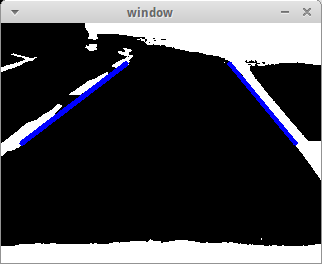
\includegraphics[width=7cm]{bv1}
\caption{Farhbahn-Erkennung}
\label{fig:bv1}
\end{figure}

\subsection{Allgemeine Idee}
\label{sec:a2idee}
Auch bei dieser Aufgabe kann die Bilderkennung in folgende Unterpunkte gegliedert werden:

\begin{enumerate}
    \item Bild laden
    \item Bild aufbereiten
    \item Fahrbahn erkennen
\end{enumerate}

In Punkt eins wird das Bild aus dem Video geladen. Die Umwandlung in ein Zwei-Pegel-Bild findet in Punkt zwei statt. Im letzten Schritt werden im Bild die Fahrbahn-Begrenzungen und Stopplinien erkannt.

\subsection{Umsetzung}
\label{sec:a2umsetzung}
Der Quellcode des Programms wurde auf zwei Dateien aufgeteilt. In der ersten befindet sich die Haupt-Routine. Diese lädt ein Bild, bereitet dieses auf, und gibt es an die zweite Datei weiter. Diese sucht nach den Markierungen und gibt die Ergebnisse zurück an das Hauptprogramm. Im folgenden werden gekürzte Quellcode-Auschnitte gezeigt. Der gesamte Quellcode ist im Internet zu finden.

\paragraph{Hauptprogramm}
Das Hauptprogramm beginnt mit dem Einlesen eines Frames. Dieses ist in Listing \ref{lst:getframe} zu sehen. In Zeile eins wird das Video geladen. Zeile zwei fordert anschließend den nächsten Frame des Videos an. In diesem Quellcode-Auszug wird lediglich ein Frame angezeigt. Im echten Programm wird dies für jedes vorhandene Bild durchgeführt.

Die Zeilen drei und vier werden verwendet um das Bild erst in ein Grauton-Bild umzuwandeln und anschließend in ein Zwei-Pegel-Bild. Dieses Zwei-Pegel-Bild wird in der letzten Zeile der Erkennungs-Logik übergeben.

\begin{lstlisting}[frame=single, float, caption={Einlesen eines Bilds}, label={lst:getframe}]
video = cv.CaptureFromFile(filepath)
frame = cv.QueryFrame(video)
cv.CvtColor(frame,framebw,cv.CV_BGR2GRAY)
cv.Threshold(framebw, framebin, 150, 255, cv.CV_THRESH_BINARY);
result = checkimage(framebin, frameoutcol)
\end{lstlisting}

Listing \ref{lst:callcheck} zeigt die Aufteilung der Logik. Hier werden sowohl für den linken und rechten Rand als auch die Stopplinie je eine Funktion aufgerufen.

\begin{lstlisting}[frame=single, float, caption={Aufruf der Fahrbahn-Erkennung}, label={lst:callcheck}]
right = checkborderright(frame, frameout)
left = checkborderleft(frame, frameout)
stop = checkstop(frame, frameout)
\end{lstlisting}

\paragraph{Fahrbahn-Begrenzung erkennen}
Die genaue Implementation der Logik soll hier der Übersicht halber nicht weiter betrachtet werden. Die Erkennung erfolgt nach einem sehr einfachen Muster:

\begin{itemize}
    \item Suche in Zeile X von Mitte bis Rand einen weißen Pixel
    \item Falls gefunden: Rand erkannt
    \item Falls nicht: Suche in nächster Zeile
\end{itemize}

Dieser Minimal-Ansatz wird durch kleine Erweiterungen etwas verbessert. So wird ein Rand nicht gewertet, wenn er nur einen Pixel breit ist. Das ändert jedoch nichts daran, dass der Algorithmus nicht stabil ist. So werden häufig noch falsche Ränder erkannt, oder der Rechte Rand als der Linke gewertet. Es zeigt jedoch gut mit welchen Mittel eine solche Lösung entworfen werden kann.

\paragraph{Stopplinien erkennen}
Die Stopplinien-Erkennung erfolgt nach einem ähnlichen Schema wie die Rand-Erkennung. So werden die Pixel in der Mitte des Bildes von unten nach oben ausgewertet. Falls ein weißer Pixel erkannt wird, wird zusätzlich überprüft ob die Linie eine gewisse horizontale Länge aufweist.

Obwohl auch dieser Algorithmus sehr einfach und nicht stabil ist, werden erstaunlich gute Ergebnisse erzielt. So werden in den meisten Fällen die Stopplinien erkannt. Auch Falsch-Positiv-Ergebnisse sind relativ selten.


\subsection{Mögliche Verbesserungen}
\label{sec:a2verbesserungen}
Wie schon bei der ersten Aufgabe ist auch dieses Projekt eher als Proof-of-Concept zu verstehen. Aus diesem Grund gibt es einige Verbesserungs-Möglichkeiten. So könnten bei der Bild-Aufbereitung komplexere Algorithmen, wie zum Beispiel ein Canny- oder Sobel-Filter, angewendet werden. Auch ein adaptiver Schwellwert für die Erstellung des Zwei-Pegel-Bilds könnte sich vorteilhaft auswirken.


%%%%%%%%%%%%%%%%%%%%%%%%%%%%%%%%%%%%%%%%%%%%%%%%%%%%%%%%%%%
% Was haben wir aus dem ganzen Kram gelernt ;-)
\section{Fazit}
\label{sec:Fazit}
Während dieser Projekte konnte ein interessanter Überblick über die Anwendung der Bildverarbeitung gewonnen werden. Dabei konnte vor allem mit verschiedenen Techniken experimentiert werden. Die Lösungen der Aufgaben sind jedoch eher als Proof-of-Concept zu sehen und würden wahrscheinlich für Produktiv-Systeme nicht ausreichen.




%%%%%%%%%%%%%%%%%%%%%%%%%%%%%%%%%%%%%%%%%%%%%%%%%%%%%%%%%%%
% Ein paar Quellenangaben...
\begin{thebibliography}{------}
\label{sec:Literatur}

%\bibitem[1]{1} \textsc{Peter Löw, Roland Pabst, Erwin Petry}: {\em Funktionale Sicherheit in der Praxis.} dpunkt.verlag, 2010.
%\bibitem[2]{2} \textsc{Jürgen Sauler, Stefan Kriso, Martina Hafner}: {\em ISO 26262 - Die zukünftige Norm zur funktionalen Sicherheit von Straßenfahrzeugen.} Online unter: \url{http://www.elektronikpraxis.vogel.de/themen/elektronikmanagement/projektqualitaetsmanagement/articles/242243/}, 2011.
%\bibitem[3]{3} \textsc{Freescale Semiconductor Inc.}: {\em ISO 26262 cuts electronics complexity risks: Pt. 1- Requirements and assessment flow.} Online unter: \url{http://eetimes.com/design/automotive-design/4236887/}, 2012.
\bibitem[1]{1} \textsc{The Mathworks Inc}: {\em Matlab Referenz.} Online unter: \url{http://www.mathworks.de/help/toolbox/images/ref/bwlabel.html}, 2012.





\end{thebibliography}





\end{document}
